%

\subsection{Proof Sketch of \cref{fact:oracle-hypothesis}}\label{sec:proof-sketch}

The primary technical result (proved in \cref{sec:impossibility-proofs}) that facilitates our results is:

%
\begin{theorem}\label{fact:interior-freedom}
Fix any \obsname{} $\covval\in\covspace$, \covname{} $j\in[\covdim]$, 
%
\radiusname{} $\inscale>0$,
\basename{} $\covdist \in \probspace(\covspace)$, 
and
\modbehaviourname{} $\modeldum:[\covval\feat{j}-\inscale, \covval\feat{j}+\inscale]\to\dataspace$.
Suppose that \cref{assn:inscale-covdist,assn:piecewise} are satisfied. 
%
For every \attname{} $\expval \in \Reals^{\datadim}$, there exists 
a \modelname{} $\model\in\modelspace$ such that for every \completename{} and \additivename{} \fielddefname{}, $\expdef(\model,\covdist,\covval)\feat{j} = \expval$, and if $\abs[0]{\covval\feat{j}-\covvaldum\feat{j}} \leq \inscale\feat{j}$ then $\model(\covvaldum) = \modeldum(\covvaldum\feat{j})$.
\end{theorem}

Equipped with \cref{fact:interior-freedom}, we use it to prove \cref{fact:oracle-hypothesis} by constructing a counterexample. For any \nullname{} $\modelspace\nullind$ and \altname{} $\modelspace\altind$, we choose $\modeldum\nullind$ and $\modeldum\altind$ satisfying the \countmodbehaviourname{} prescribed by the \nullname{} and \altname{} respectively. For example, in the recourse setting, $\modeldum\nullind$ may be increasing in the \covname{} while $\modeldum\altind$ is decreasing.
%
Then, by \cref{fact:interior-freedom}, we can construct $\model\nullind$ and $\model\altind$ that locally agree with $\modeldum\nullind$ and $\modeldum\altind$ respectively, yet receive the same \covname{} \attname{}. Consequently, any \oraclehyptestname{} that relies on only the \covname{} \attname{} to draw conclusions cannot distinguish between $\model\nullind$ and $\model\altind$, and hence has been provided no additional information to do better than random guessing.
While a single counterexample is sufficient to prove \cref{fact:oracle-hypothesis}, the proof of \cref{fact:interior-freedom} reveals that we can actually find uncountably many \modelnames{} that work as counterexamples, which has important implications for practical settings.
We demonstrate this in our on-average results (\cref{sec:average-behaviour}) and experiments (\cref{sec:experiments}).

We visualize the intuition behind this result in \cref{fig:attribution}, where we show (a) \modelnames{} can behave very differently and all receive the same attribution and (b) \modelnames{} can be identical in a local neighbourhood of interest yet receive very different attribution. 
%
Critically, our counterexamples are very simple (piecewise linear in the proof, piecewise quadratic for smooth visualization in \cref{fig:attribution}), and hence easily realized by neural networks.
Finally, since \fielddefnames{} provide only a summary of the \modelname{}, it is clear that one can always find \emph{some} example of two different \modelnames{} that receive the same \attname{}.
The primary insight that enables our results is that we can always find \modelnames{} that \emph{differ in exactly the way that we wish to test} yet receive the same \attname{}. The next natural question is: how does this result extend to \downtasknames{} that practitioners care about?


%
%
%
%
%
%
%
%
%
%
%
%
%

\begin{figure}
\centering
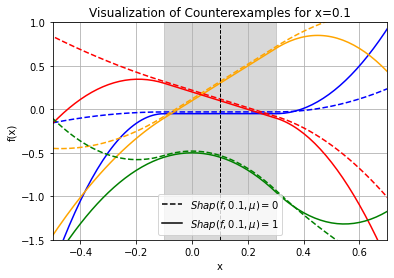
\includegraphics[scale=0.6]{figure-files/joint-att.png}
    \caption{Each line represents a different one-dimensional \modelname{}. For $\covval=0.1$ and $\covdist=\uniformdist(-1,1)$, dashed lines receive \shap{}$(\model,\covval,\covdist)=0$ while solid lines receive \shap{}$(\model,\covval,\covdist)=1$. The behaviour of models with the same colour is identical within the shaded region, which denotes the neighbourhood $(\covval-\inscale,\covval+\inscale)$ for $\inscale=0.2$. \modelNames{} can behave very differently and all receive the same \attname{} (e.g., all dashed lines) and \modelnames{} can be identical in a neighbourhood yet receive very different \attname{} within that neighbourhood (e.g., lines with the same colour). }
    \label{fig:attribution}
\end{figure}
%
%
%
%

%
%
%
%
%